%%
%% This is file `mathexample.tex',
%% generated with the docstrip utility.
%%
%% The original source files were:
%%
%% texpower-doc.dtx  (with options: `mathexample,mathexample-src,end')
%% 
%% --------------------------------------------------------------
%% TeXPower bundle - dynamic online presentations with LaTeX
%% Copyright (C) 1999-2004 Stephan Lehmke
%% Copyright (C) 2003-2005 Hans Fredrik Nordhaug
%% 
%% This program is free software; you can redistribute it and/or
%% modify it under the terms of the GNU General Public License
%% as published by the Free Software Foundation; either version 2
%% of the License, or (at your option) any later version.
%% 
%% This program is distributed in the hope that it will be useful,
%% but WITHOUT ANY WARRANTY; without even the implied warranty of
%% MERCHANTABILITY or FITNESS FOR A PARTICULAR PURPOSE.  See the
%% GNU General Public License for more details.
%% --------------------------------------------------------------
%% 
%% The list of all files belonging to the TeXPower bundle is
%% given in the file `00readme.txt'.
%% 
\ProvidesFile{talk.tex}%
      [2005/04/07 TeXPower example file]
%-----------------------------------------------------------------------------------------------------------------
%
% Math example for the package texpower.sty.
%
%-----------------------------------------------------------------------------------------------------------------
% Enable all color emphasis and highlighting options. Use white background and slifonts.

\PassOptionsToPackage{coloremph,colormath,colorhighlight,darkbackground}{texpower}

% Input the generic preamble.

%\input{__TPpreamble}
\documentclass[12pt,letterpaper,landscape,KOMA,smallheadings,calcdimensions,display]{powersem}

\usepackage{tpslifonts}
%-----------------------------------------------------------------------------------------------------------------
% We load hyperref and fixseminar which fixes some problems with seminar.
%
\usepackage[ps2pdf,plainpages=false,bookmarksopen,colorlinks,pdfpagemode=FullScreen]{hyperref}
\usepackage{seminar}
\usepackage{fixseminar}

%-----------------------------------------------------------------------------------------------------------------
% Finally, the texpower package is loaded.
%
\usepackage{texpower}
\usepackage{soul}


% We write some aligned equations.

\usepackage{amsmath}
\usepackage{amssymb}
\usepackage{relsize}
\usepackage[pdftex]{graphicx}
% Make nested braces grow.
\delimitershortfall-1sp

%-----------------------------------------------------------------------------------------------------------------
% Finally, everything is set up. Here we go...
%

\input{latexdefs.tex}


%-----------------------------------------------------------------------------------------------------------------
% Set slide margins rather small for maximum use of space. 
%
\renewcommand{\slidetopmargin}{5mm}
\renewcommand{\slidebottommargin}{5mm}

\renewcommand{\slideleftmargin}{5mm}
\renewcommand{\sliderightmargin}{5mm}
\renewcommand\section{\@startsection{section}{1}{\z@}%
  {-1.5ex\@plus -1ex \@minus -.5ex}%
  {.5ex \@plus .2ex}%
  {\raggedsection\normalfont\size@section\sectfont}}

\renewcommand\subsection{\@startsection{subsection}{2}{\z@}%
  {-1.25ex\@plus -1ex \@minus -.2ex}%
  {.5ex \@plus .2ex}%
  {\raggedsection\normalfont\size@subsection\sectfont}}

\renewcommand\subsubsection{\@startsection{subsubsection}{3}{\z@}%
  {-1.25ex\@plus -1ex \@minus -.2ex}%
  {.5ex \@plus .2ex}%
  {\raggedsection\normalfont\size@subsubsection\sectfont}}

\renewcommand\paragraph{\@startsection{paragraph}{4}{\z@}%
  {1.25ex \@plus1ex \@minus.2ex}%
  {-1em}%
  {\raggedsection\normalfont\size@paragraph\sectfont}}

\def\slideitemsep{.5ex plus .3ex minus .2ex}



\newcommand{\sunu}{SU(N) \times U(1)}
\newcommand{\aU}{a^{\rm U(1)}}
\newcommand{\aN}{a^{\rm SU(N)}}
\newcommand{\lU}{\lambda^{\rm U(1)}}
\newcommand{\lN}{\lambda^{\rm SU(N)}}
\newcommand{\Tr}{{\rm Tr\,}}
\newcommand{\bxir}{\ov{\xi}{}_R}
\newcommand{\bxil}{\ov{\xi}{}_L}
\newcommand{\xir}{\xi_R}
\newcommand{\xil}{\xi_L}
\newcommand{\bzl}{\ov{\zeta}{}_L}
\newcommand{\bzr}{\ov{\zeta}{}_R}
\newcommand{\zr}{\zeta_R}
\newcommand{\zl}{\zeta_L}
\newcommand{\nbar}{\ov{n}}



\begin{document}

%%%%%%%%%%%%%%%%%%%%%%%%%%%%%%%%%%%%%%%%%%%%%%%%%%%%%%%%%%%%%%%%%%%%%%%%%%%%%%%%%%%%%
%%%%%%%%%%%%%%%%%%%%%%%%%%%%%%%%%%%%%%%%%%%%%%%%%%%%%%%%%%%%%%%%%%%%%%%%%%%%%%%%%%%%%
\begin{slide}
%-----------------------------------------------------------------------------------------------------------------
%
\vspace*{\fill}
\title{Non-abelian Vortices in $\mathcal{N}=1$ SQCD}
\author{Pavel A. Bolokhov\\
\tiny
~~~~University of Pittsburgh ~~$\bullet$~~ St.Petersburg State University}
\date{}
\maketitle
\vspace*{\fill}
\end{slide}


%%%%%%%%%%%%%%%%%%%%%%%%%%%%%%%%%%%%%%%%%%%%%%%%%%%%%%%%%%%%%%%%%%%%%%%%%%%%%%%%%%%%%
%%%%%%%%%%%%%%%%%%%%%%%%%%%%%%%%%%%%%%%%%%%%%%%%%%%%%%%%%%%%%%%%%%%%%%%%%%%%%%%%%%%%%
\begin{slide}
%\liststepwise[\let\hidestepcontents=\hidedimmed\let\activatestep=\highlightenhanced]
%{
%	\step
	{
	Confinement is customary thought of as medium where (chromo)electric charges are
	bound by flux tubes via condensation of monopoles. 
	}

%	\step
	{
	A number of theories have been proposed, such as the Seiberg-Witten theory, which
	are shown to have confinement.
	}

%	\step
	{
	However, in these theories, confinement is essentially abelian.
	This has problems with our experience with QCD.
	The low-energy group is $ U(1)^{N-1} $ which leads to the existence of $ N-1 $ Abelian
	strings, and therefore $ N-1 $ infinite towers of mesons. 
	}

%	\step
	{
	In real-world QCD confinement is \emph{non-abelian}.
	}
%}	

\end{slide}

%%%%%%%%%%%%%%%%%%%%%%%%%%%%%%%%%%%%%%%%%%%%%%%%%%%%%%%%%%%%%%%%%%%%%%%%%%%%%%%%%%%%%
%%%%%%%%%%%%%%%%%%%%%%%%%%%%%%%%%%%%%%%%%%%%%%%%%%%%%%%%%%%%%%%%%%%%%%%%%%%%%%%%%%%%%
\begin{slide}

	Certain supersymmetry SQCD scenarios allow condensation of quarks to cause
	confinement of the monopoles

\begin{center}
\textcolor{yellow}{
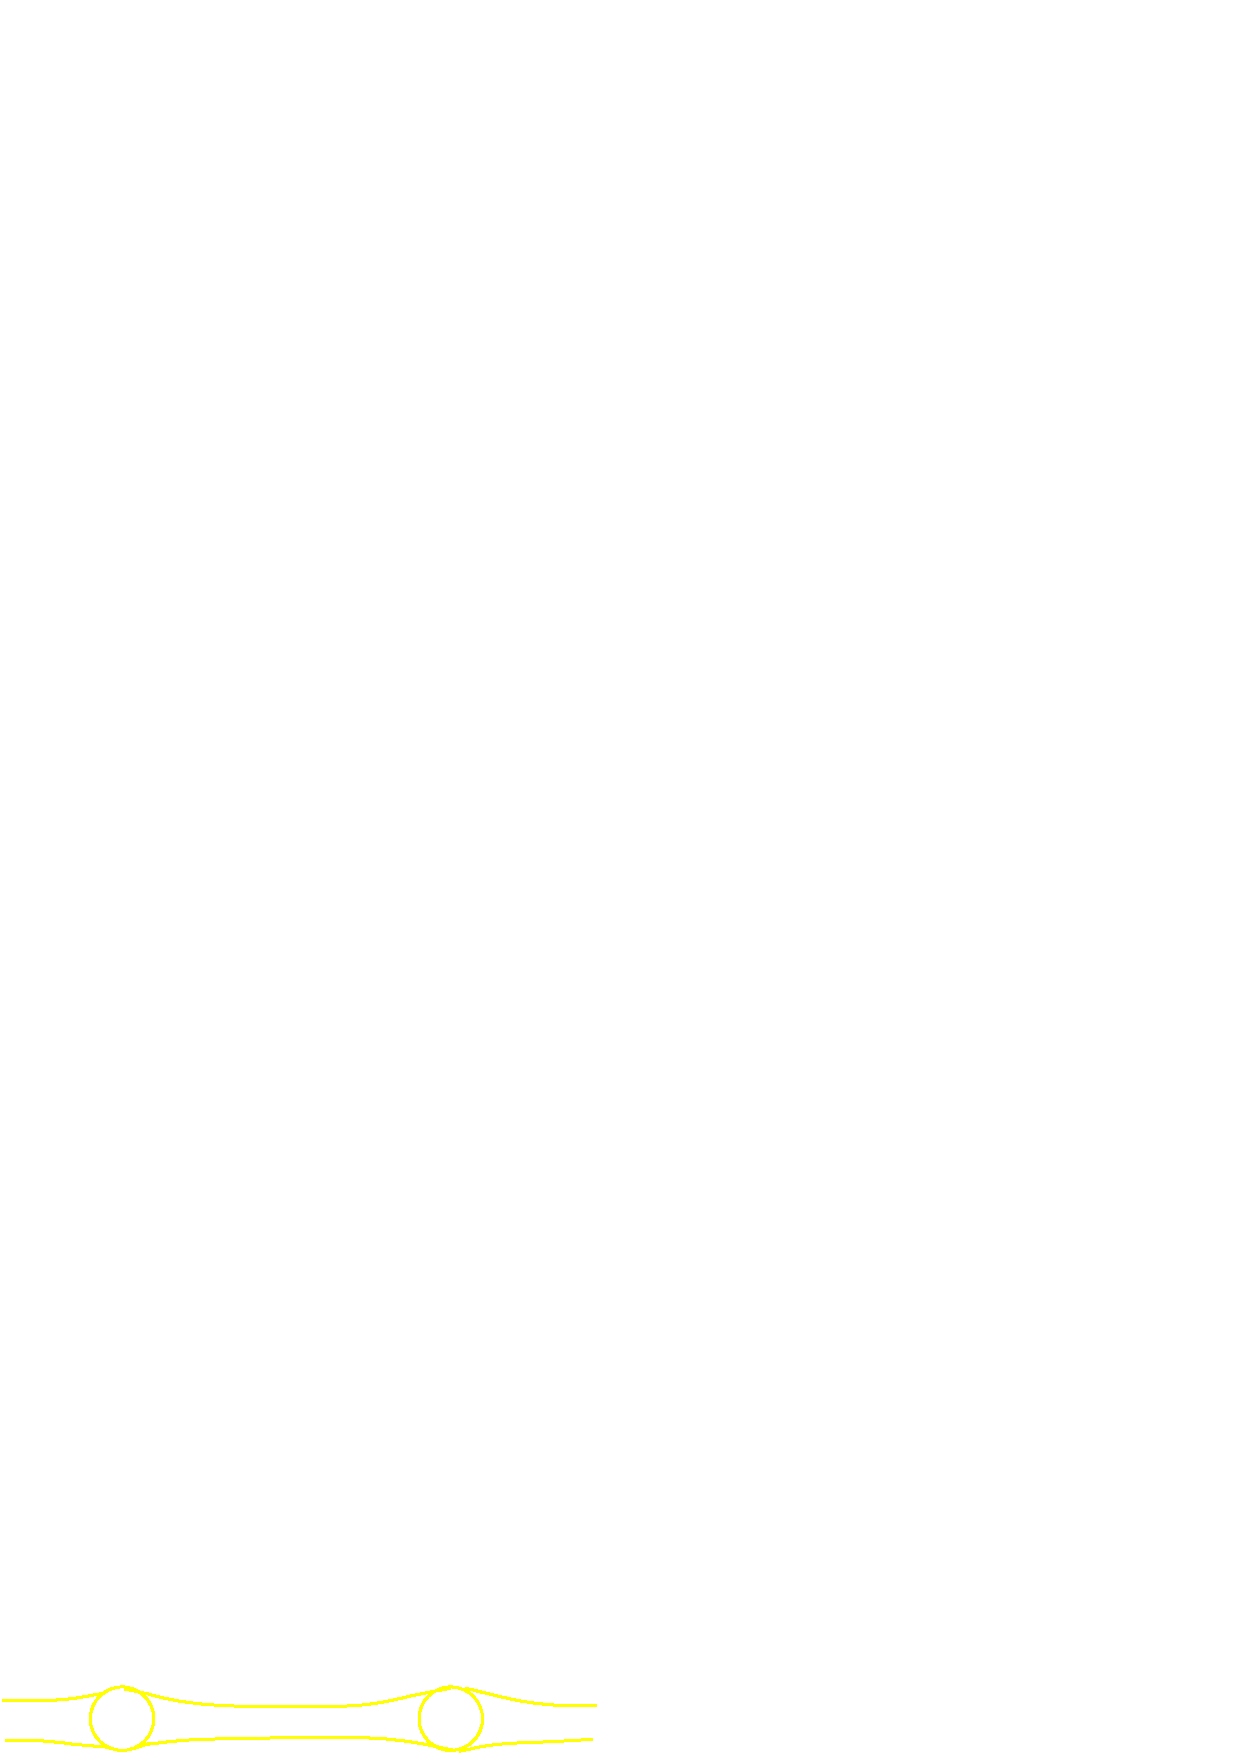
\includegraphics[width=5.0cm]{str_mon.pdf}
}
\end{center}

	Vortex strings are allowed to end on a monopole which they therefore confine.
	The low-energy dynamics of these strings is described by an effective 2-dimensional
	worldsheet theory

	The strings represent the vacua of this theory, while the monopoles play the role
	of \emph{kinks} of the worldsheet theory

	For the study of confinement of monopoles, therefore, it is instructive to investigate
	the dynamics of 2-dim (typically CP(N-1)) effective worldsheet theory
\end{slide}


%%%%%%%%%%%%%%%%%%%%%%%%%%%%%%%%%%%%%%%%%%%%%%%%%%%%%%%%%%%%%%%%%%%%%%%%%%%%%%%%%%%%%
%%%%%%%%%%%%%%%%%%%%%%%%%%%%%%%%%%%%%%%%%%%%%%%%%%%%%%%%%%%%%%%%%%%%%%%%%%%%%%%%%%%%%
\begin{slide}
\vspace*{\fill}
	We consider the $ \mc{N}=2 $ SQCD theory with a gauge group $\sunu$.
	
	Supposedly it emerges from $ SU(N+1) $ broken down to $\sunu$ at the scale
\[
	m ~~ \gg ~~ \Lambda_{SU(N+1)}~
\]

	Later we break $ \mc{N}=2 $ supersymmetry to $ \mc{N}=1 $.
\vspace*{\fill}
\end{slide}


%%%%%%%%%%%%%%%%%%%%%%%%%%%%%%%%%%%%%%%%%%%%%%%%%%%%%%%%%%%%%%%%%%%%%%%%%%%%%%%%%%%%%
%%%%%%%%%%%%%%%%%%%%%%%%%%%%%%%%%%%%%%%%%%%%%%%%%%%%%%%%%%%%%%%%%%%%%%%%%%%%%%%%%%%%%
\begin{slide}
\vspace*{3.0cm}
%\relsize{+8}  
\usefont{T1}{ptm}{m}{n}\fontsize{40pt}{40pt}\selectfont
\begin{center} 
	$\mc{N}=2$ SQCD 
\end{center}
	
\vspace*{\fill}
\end{slide}


%%%%%%%%%%%%%%%%%%%%%%%%%%%%%%%%%%%%%%%%%%%%%%%%%%%%%%%%%%%%%%%%%%%%%%%%%%%%%%%%%%%%%
%%%%%%%%%%%%%%%%%%%%%%%%%%%%%%%%%%%%%%%%%%%%%%%%%%%%%%%%%%%%%%%%%%%%%%%%%%%%%%%%%%%%%
\begin{slide}
	The content of the $ \mc{N}=2 $ SQCD is as follows:

	The gauge multiplet includes $ \mc{N}=1 $ gauge multiplets
\begin{align*}
	&W_\alpha^{\rm U(1)}  \qquad\owns\qquad A_\mu^{\rm U(1)}~~\qquad  \lambda^{1\,\rm U(1)} \\
	&W_\alpha^{\rm SU(N)}	\qquad\owns\qquad A_\mu^{\rm SU(N)}~~\qquad \lambda^{1\, \rm SU(N)}
\end{align*}
	and the chiral multiplets
\begin{align*}
	&\mc{A}^{\rm U(1)}	\qquad\owns\qquad a^{\rm U(1)}~~\qquad \lambda^{2\,\rm U(1)} \\
	&\mc{A}^{\rm SU(N)}	\qquad\owns\qquad a^{\rm SU(N)}~~\qquad \lambda^{2\,\rm SU(N)}
\end{align*}
	Matter multiplets, in $ N_F = N $ quantity
\begin{align*}
	&Q^{kA}		\qquad\owns\qquad	q^{kA}~~\qquad   \psi^{kA} \\
	&\wt{Q}{}_{Ak}		\qquad\owns\qquad	\wt{q}_{Ak}~~\qquad  \wt{\psi}{}_{Ak}~.
\end{align*}

\end{slide}

%%%%%%%%%%%%%%%%%%%%%%%%%%%%%%%%%%%%%%%%%%%%%%%%%%%%%%%%%%%%%%%%%%%%%%%%%%%%%%%%%%%%%
%%%%%%%%%%%%%%%%%%%%%%%%%%%%%%%%%%%%%%%%%%%%%%%%%%%%%%%%%%%%%%%%%%%%%%%%%%%%%%%%%%%%%
\begin{slide}
	One also introduces Fayet-Iliopoulos terms:
\begin{align*}
	\mathlarger{\mathlarger{\mc{W}_A }} & 
		{\mathlarger{~~=~~ -\,\frac{N}{2\sqrt{2}}\,\xi\mc{A}^{\rm U(1)}}} ~,   
		\qquad \text{--  F-term} \\
	 \xi & ~~=~~ \xi_1 ~-~ i\xi_2~,
\end{align*}
	or alternatively (and the only one for $\mc{N}=1$)
\[
\mathlarger{
	\mathlarger{\mc{L}} ~~\supset~~  -\frac{N}{2} \int d^4\theta~ \xi_3 V^{\rm U(1)}
	}~, \qquad \text{-- D-term.}
\]
	
	$\xi_1$, $\xi_2$ and $\xi_3$ form an $SU_R(2)$ triplet of ``generalized FI parameters'', and
	are completely equivalent for $ \mc{N}=2 $ supersymmetry

	they trigger condensation of quarks

	condensation of quarks leads to formation of flux tubes
\end{slide}


%%%%%%%%%%%%%%%%%%%%%%%%%%%%%%%%%%%%%%%%%%%%%%%%%%%%%%%%%%%%%%%%%%%%%%%%%%%%%%%%%%%%%
%%%%%%%%%%%%%%%%%%%%%%%%%%%%%%%%%%%%%%%%%%%%%%%%%%%%%%%%%%%%%%%%%%%%%%%%%%%%%%%%%%%%%
\begin{slide}
	The potential of this theory is
\begin{align*}
%
	V(q^A,\wt{q}{}_A,a^a,a) &~~=~~
			\frac{g_2^2}{2} \left( \frac{1}{g_2^2}f^{abc}\ov{a}{}^b a^c  ~+~
						\ov{q}{}_A T^a q^A  - \wt{q}{}_A T^a \ov{\wt{q}}{}^A \right)^2 \\
%
	& ~~+~~ \frac{g_1^2}{8}\, \left(\ov{q}{}_A q^A ~-~ \wt{q}{}_A\ov{\wt{q}}{}^A ~-~ N\,\xi_3 \right)^2 \\
%
	& ~~+~~ 2\,g_2^2 \left| \wt{q}{}_A T^a q^A \right|^2 ~+~
		\frac{g_1^2}{2} \left| \wt{q}_A q^A ~-~ \frac{N}{2}\, \xi \right|^2 \\
%
	& ~~+~~ \frac{1}{2} \sum_{A=1}^N \Biggl\{ \left|\left(a ~+~ \sqrt{2}m_A ~+~ 2T^a a^a\right)q^A\right|^2 \\
%	
	& \phantom{\frac{1}{2}\sum_{A=1}^N \Biggl\{ } ~~+~~
		\left| \left( a ~+~ \sqrt{2}m_A ~+~ 2T^a a^a\right) \ov{\wt{q}}^A \right|^2 \Biggr\}~.
\end{align*}

\end{slide}


%%%%%%%%%%%%%%%%%%%%%%%%%%%%%%%%%%%%%%%%%%%%%%%%%%%%%%%%%%%%%%%%%%%%%%%%%%%%%%%%%%%%%
%%%%%%%%%%%%%%%%%%%%%%%%%%%%%%%%%%%%%%%%%%%%%%%%%%%%%%%%%%%%%%%%%%%%%%%%%%%%%%%%%%%%%
\begin{slide}

	The potential causes condensation of quarks and of the adjoint matter
\[
	\frac{1}{2}a ~~+~~ T^a a^a  ~~=~~ \begin{pmatrix}
					  	0 & \ldots & 0 \\
						\ldots & \ldots & \ldots \\
						0 & \ldots & 0 
					  \end{pmatrix}
\]
	For quarks one can choose the Colour-Flavour Locked form
\[
	\left\langle q^{kA} \right\rangle ~~=~~ \left\langle \ov{\wt{q}}{}^{kA} \right\rangle ~~=~~ 
			\sqrt{\frac{\xi}{2}} \begin{pmatrix}
					     	1  & \ldots  & 0 \\
						\ldots & \ldots & \ldots \\
						0 & \ldots &  1
					     \end{pmatrix}
\]
\end{slide}

%%%%%%%%%%%%%%%%%%%%%%%%%%%%%%%%%%%%%%%%%%%%%%%%%%%%%%%%%%%%%%%%%%%%%%%%%%%%%%%%%%%%%
%%%%%%%%%%%%%%%%%%%%%%%%%%%%%%%%%%%%%%%%%%%%%%%%%%%%%%%%%%%%%%%%%%%%%%%%%%%%%%%%%%%%%
\begin{slide}
\vspace*{\fill}
	This way the diagonal symmetry is unbroken
\[
	U_C(N) ~\times~ SU_F(N)  ~~\to~~ SU_{C+F}(N)~.
\]

	The gauge bosons acquire a mass
\[
	M_{\rm SU(N)} ~~=~~ g_2 \sqrt{\xi}
\]
	and
\[
	M_{\rm U(1)} ~~=~~ g_1 \sqrt{\frac{N}{2}\xi}
\]
\vspace*{\fill}
\end{slide}

%%%%%%%%%%%%%%%%%%%%%%%%%%%%%%%%%%%%%%%%%%%%%%%%%%%%%%%%%%%%%%%%%%%%%%%%%%%%%%%%%%%%%
%%%%%%%%%%%%%%%%%%%%%%%%%%%%%%%%%%%%%%%%%%%%%%%%%%%%%%%%%%%%%%%%%%%%%%%%%%%%%%%%%%%%%
\begin{slide}
	The $ Z_N $ string solution

\begin{center}
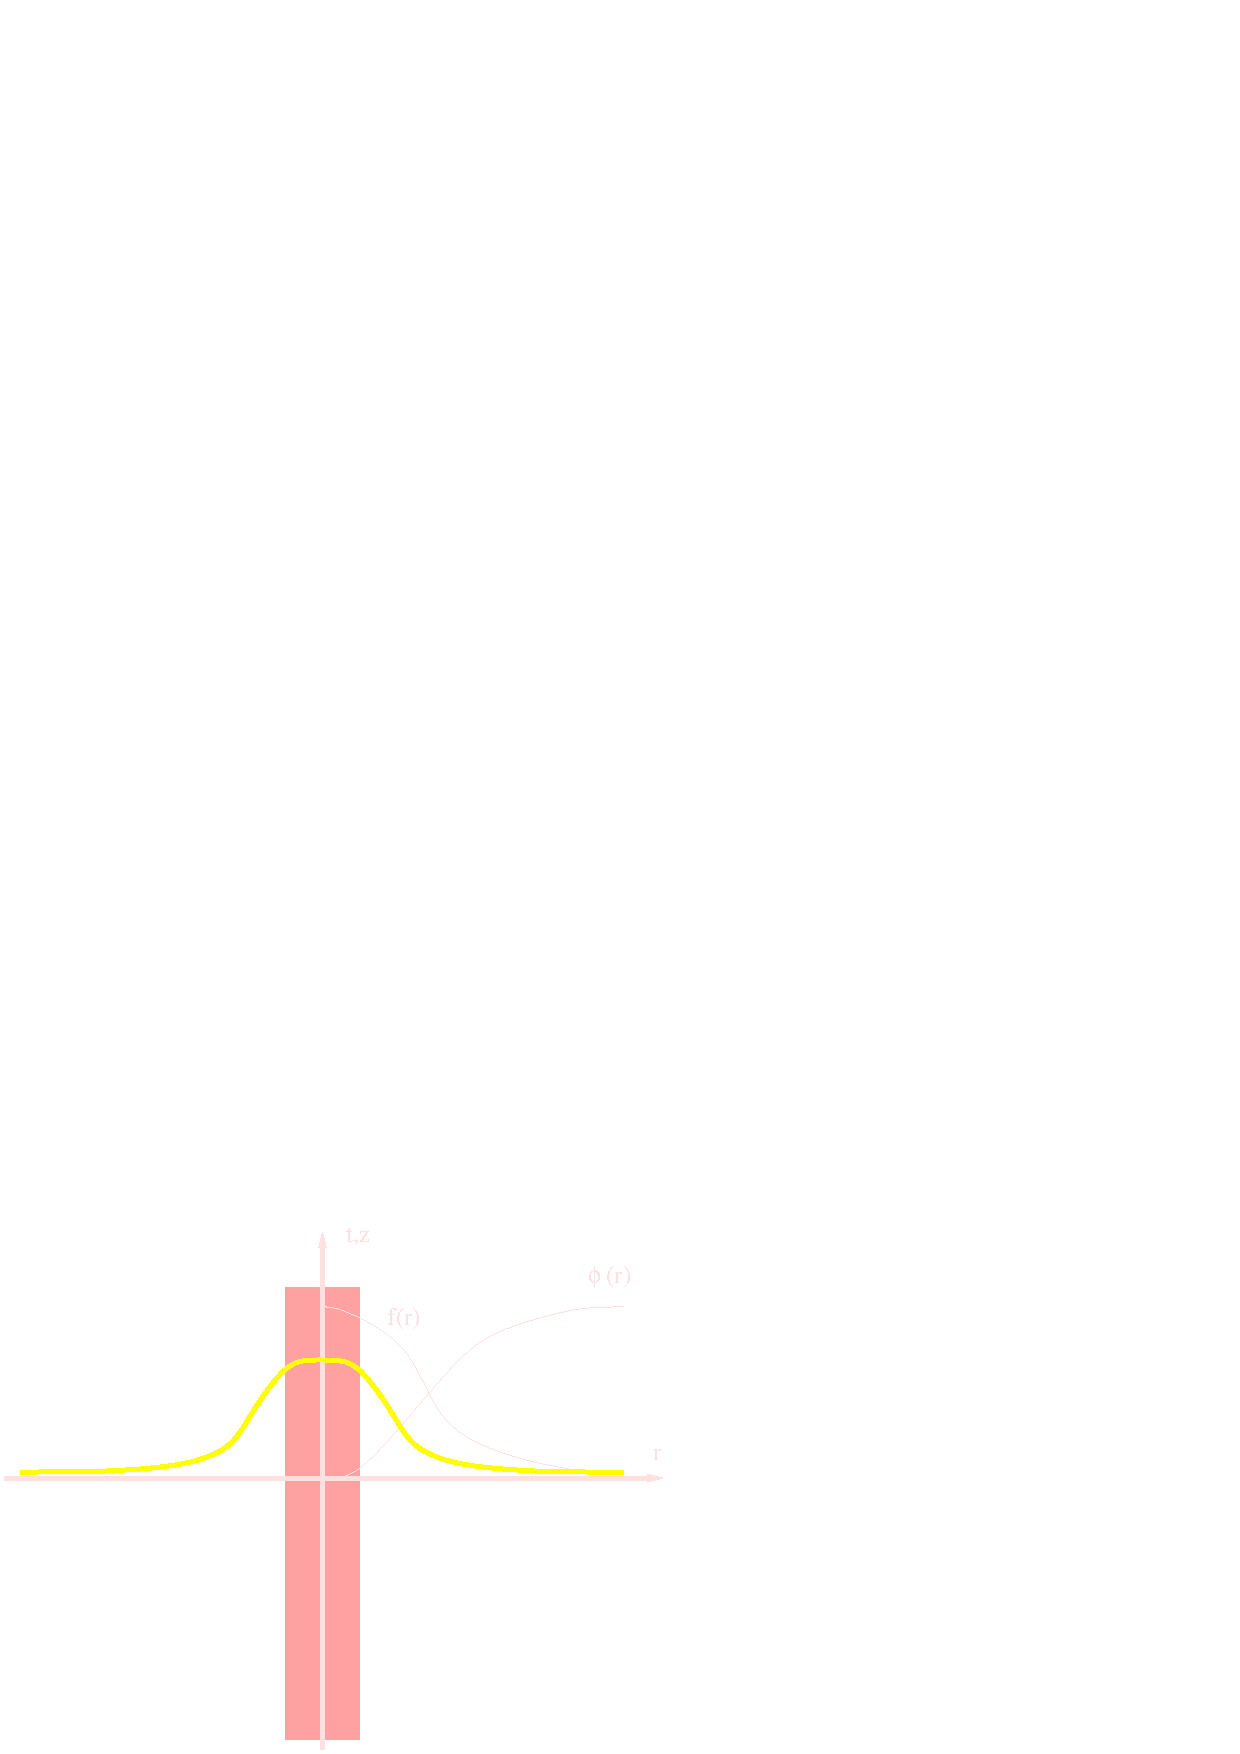
\includegraphics[width=9.0cm]{string.pdf}
\end{center}

\end{slide}


%%%%%%%%%%%%%%%%%%%%%%%%%%%%%%%%%%%%%%%%%%%%%%%%%%%%%%%%%%%%%%%%%%%%%%%%%%%%%%%%%%%%%
%%%%%%%%%%%%%%%%%%%%%%%%%%%%%%%%%%%%%%%%%%%%%%%%%%%%%%%%%%%%%%%%%%%%%%%%%%%%%%%%%%%%%
\begin{slide}
	The $ Z_N $ string solution
\begin{align*}
%
	\varphi ~~=~~ & \lgr \begin{matrix}
			   	\phi_2(r)  & 0  & \ldots & 0 \\
				\ldots  &  \ldots & \ldots & \ldots \\
				0  & \ldots      & \phi_2(r) &  0 \\
				0  & 0           & \ldots  &   e^{i\alpha} \phi_1(r) 
			   \end{matrix}        \rgr     \\
%
	A_i^{\rm SU(N)} ~~=~~ \frac{1}{N} & \lgr \begin{matrix}
					          	1  & \ldots & 0 & 0 \\
						  	\ldots & \ldots & \ldots & \ldots \\
							0  & \ldots  & 1  &  0 \\
							0  & 0   & \ldots  &  - (N-1) 
					         \end{matrix} \rgr  \times \\
%
			&	\qquad\qquad\qquad\qquad     \times(\p_i \alpha) \lgr  -1 ~+~ f_{NA}(r) \rgr  \\
%
	A_i^{\rm U(1)} ~~=~~ & \frac{1}{N} (\p_i \alpha) \lgr 1 ~-~ f(r) \rgr
%			A_0^{\rm U(1)} ~~=~~ A_0^{\rm SU(N)} ~~=~~ 0~.
\end{align*}

\end{slide}

%%%%%%%%%%%%%%%%%%%%%%%%%%%%%%%%%%%%%%%%%%%%%%%%%%%%%%%%%%%%%%%%%%%%%%%%%%%%%%%%%%%%%
%%%%%%%%%%%%%%%%%%%%%%%%%%%%%%%%%%%%%%%%%%%%%%%%%%%%%%%%%%%%%%%%%%%%%%%%%%%%%%%%%%%%%
\begin{slide}
\vspace*{\fill}
	The string solution breaks
\[
	\frac{SU(N)}
            {SU(N-1) \times U(1)}         ~~\sim~~  CP(N-1)~\text.
\]

	The string possesses orientational moduli $ n^l $, in terms of which the
	bosonic part of the CP(N-1) action reads
\[
	S^{1+1} ~~=~~ \frac{4\pi}{g_2^2} \int dt\, dz \lgr  
			\left|\p n \right|^2  ~+~
			\left( \ov{n}\, \p_k\, n \right)^2  \rgr \text.
\]
\vspace*{\fill}
\end{slide}

%%%%%%%%%%%%%%%%%%%%%%%%%%%%%%%%%%%%%%%%%%%%%%%%%%%%%%%%%%%%%%%%%%%%%%%%%%%%%%%%%%%%%
%%%%%%%%%%%%%%%%%%%%%%%%%%%%%%%%%%%%%%%%%%%%%%%%%%%%%%%%%%%%%%%%%%%%%%%%%%%%%%%%%%%%%
\begin{slide}
	Later we will introduce $ \mc{N}=2 $ $ \to $ $ \mc{N} = 1 $ supersymmetry breaking, in order
	to get closer to the real world, via a deformation
\[
	\mc{W}_{3+1} ~~=~~ \sqrt{\frac{N}{2}}\,\frac{\mu}{2}\, \mc{A}^2 ~~+~~ \frac{\mu}{2}\,\left(\mc{A}^a\right)^2 
\] 
	and via introduction of a meson-like ``mass'' field $M$
\begin{align*}
	& \mc{W}_M ~~=~~ QM\wt{Q}~\text{,}\qquad \\
	& \mc{L}_M ~~=~~ \frac{1}{h} \left|\p_\mu M^0\right|^2 ~+~ \frac{1}{h}\left|\p_\mu M^a\right|^2~\text{.}
\end{align*}

	These modifications, change the CP(N-1) model. 

	Our goal will be to find out the changes of the CP(N-1) model.
\end{slide}


%%%%%%%%%%%%%%%%%%%%%%%%%%%%%%%%%%%%%%%%%%%%%%%%%%%%%%%%%%%%%%%%%%%%%%%%%%%%%%%%%%%%%
%%%%%%%%%%%%%%%%%%%%%%%%%%%%%%%%%%%%%%%%%%%%%%%%%%%%%%%%%%%%%%%%%%%%%%%%%%%%%%%%%%%%%
\begin{slide}
\vspace*{\fill}
	The hierarchy of scales is taken as follows:
\[
	\Lambda_{CP(N-1)} \sim \Lambda_{SU(N)} ~~\ll~~ \sqrt{\xi} ~~\ll~~ |\Delta m|
\]

	The gauge coupling is frozen below the squark condensate scale $\sqrt{\xi}$ and therefore
	below this scale one is at weak coupling
\vspace*{\fill}
\end{slide}

\begin{slide}
	When $ |\Delta m | $ becomes  $ ~\sim~ \sqrt{\xi}$, flux tubes form, whose 
	tension is smaller than the mass of the monopole:
\[
	M_M  ~~\sim~~ \frac{1}{g_2^2}|\Delta m| ~~\gg~~  \sqrt{T} ~\sim~ \sqrt{\xi}~\text{.}
\]

	This corresponds to weakly confined monopoles
\begin{center}
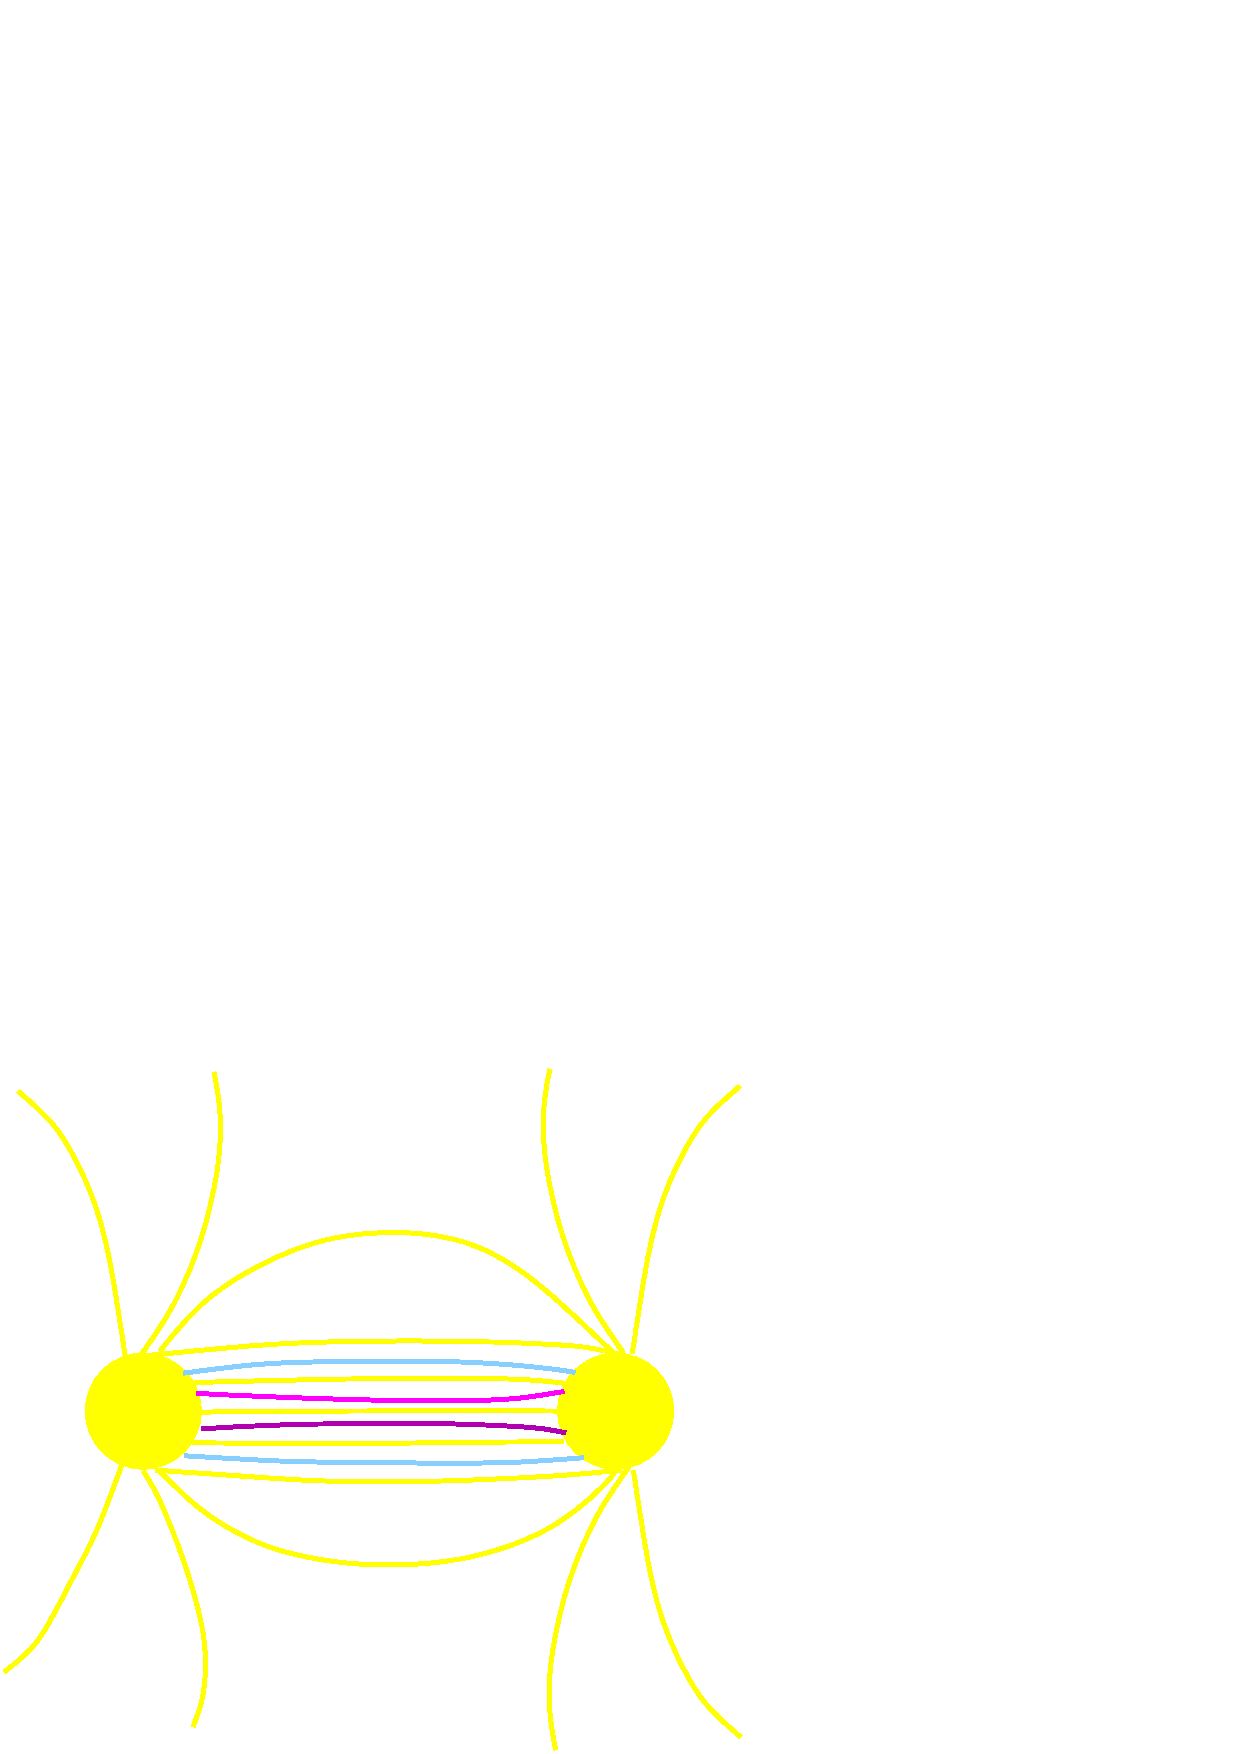
\includegraphics[width=5.0cm]{weak_conf.pdf}
\end{center}

\end{slide}

%%%%%%%%%%%%%%%%%%%%%%%%%%%%%%%%%%%%%%%%%%%%%%%%%%%%%%%%%%%%%%%%%%%%%%%%%%%%%%%%%%%%%
%%%%%%%%%%%%%%%%%%%%%%%%%%%%%%%%%%%%%%%%%%%%%%%%%%%%%%%%%%%%%%%%%%%%%%%%%%%%%%%%%%%%%
\begin{slide}
	
	Further lowering $ |\Delta m| $ increases the size of the monopole
	past the size of the core of the string attached to it --- confinement,
	in quasiclassical regime 

	As now $ |\Delta m| $ is taken to $ \Lambda_{CP(N-1)} $ and below to zero,
	the size of the monopole grows and classically explodes

	Classical treatment is unapplicable here, this is a highly quantum regime

\begin{center}
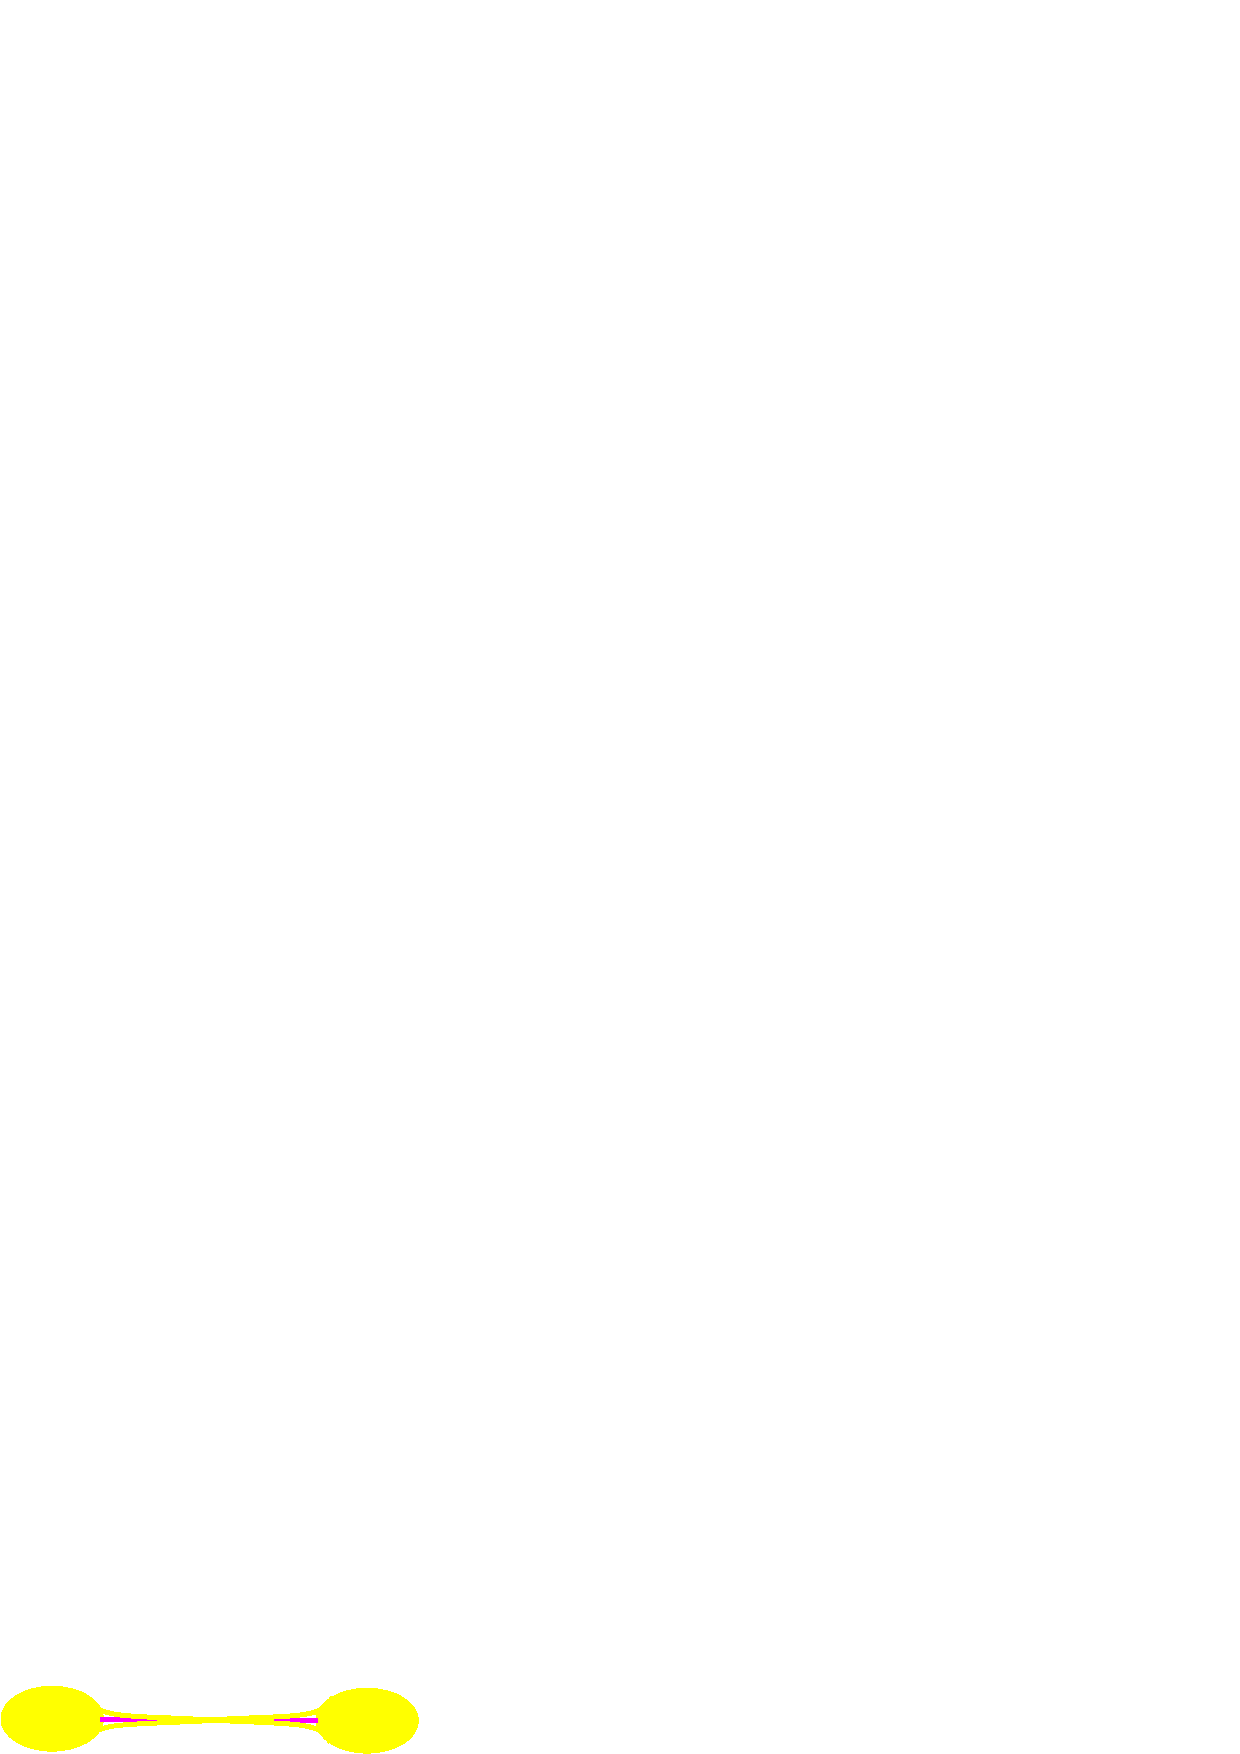
\includegraphics[width=5.0cm]{quant_conf.pdf}
\end{center}

	However, monopoles are seen as \emph{kinks} on the worldsheet theory
	interpolating between vacua which correspond to highly quantum strings

\end{slide}

%%%%%%%%%%%%%%%%%%%%%%%%%%%%%%%%%%%%%%%%%%%%%%%%%%%%%%%%%%%%%%%%%%%%%%%%%%%%%%%%%%%%%
%%%%%%%%%%%%%%%%%%%%%%%%%%%%%%%%%%%%%%%%%%%%%%%%%%%%%%%%%%%%%%%%%%%%%%%%%%%%%%%%%%%%%
\begin{slide}
\vspace*{3.0cm}
%\relsize{+8}  
\usefont{T1}{ptm}{m}{n}\fontsize{40pt}{40pt}\selectfont
\begin{center} 
	$\mc{N}=1$ SQCD 
\end{center}
	
\vspace*{\fill}
\end{slide}

%%%%%%%%%%%%%%%%%%%%%%%%%%%%%%%%%%%%%%%%%%%%%%%%%%%%%%%%%%%%%%%%%%%%%%%%%%%%%%%%%%%%%
%%%%%%%%%%%%%%%%%%%%%%%%%%%%%%%%%%%%%%%%%%%%%%%%%%%%%%%%%%%%%%%%%%%%%%%%%%%%%%%%%%%%%
\begin{slide}
\vspace*{\fill}
	To break supersymmetry to $ \mc{N}=1 $, we introduce soft mass terms for the
	adjoint chiral multiplets
\[
	\mc{W}_{3+1} ~~=~~ \sqrt{\frac{N}{2}}\,\frac{\mu}{2}\, \mc{A}^2 ~~+~~ \frac{\mu}{2}\,\left(\mc{A}^a\right)^2 
\] 

	One is tempted to take $ \mu \to \infty $.
	The problem arises, however, that $ \mc{N}=1 $ SQCD has a Higgs branch, and, correspondingly,
	massless states, and an infrared problem develops:

	\emph{the BPS strings become infinitely thick $ \sim~ \mu_/\xi $}.

	CP(N-1) description breaks down
\vspace*{\fill}	
\end{slide}


%%%%%%%%%%%%%%%%%%%%%%%%%%%%%%%%%%%%%%%%%%%%%%%%%%%%%%%%%%%%%%%%%%%%%%%%%%%%%%%%%%%%%
%%%%%%%%%%%%%%%%%%%%%%%%%%%%%%%%%%%%%%%%%%%%%%%%%%%%%%%%%%%%%%%%%%%%%%%%%%%%%%%%%%%%%
\begin{slide}
\vspace*{\fill}
	To cure this, an \emph{\it M model} is introduced

	Quarks are given a {\it dynamical} mass
\[
	\mc{L}_{\rm quark} ~~=~~ \int d^2\theta\, d^2\ov{\theta}\,  \frac{2}{h} {\rm Tr} \ov{M}M  ~~+~~
			\int d^2\theta  \, Q M\wt{Q} ~~+~~ \text{h.c.}
\]
	
	One now has two supersymmetry breaking parameters: $ \mu $ and $ h $.

	The meson field $ M $ is more natural from the Seiberg's duality standpoint.
	This field \emph{lifts} the Higgs branch
	
	This model is {\it not} the same as Seiberg's theory: gauge group is different, the
	presence of FI $D$-term, {it etc}
\vspace*{\fill}
\end{slide}

%%%%%%%%%%%%%%%%%%%%%%%%%%%%%%%%%%%%%%%%%%%%%%%%%%%%%%%%%%%%%%%%%%%%%%%%%%%%%%%%%%%%%
%%%%%%%%%%%%%%%%%%%%%%%%%%%%%%%%%%%%%%%%%%%%%%%%%%%%%%%%%%%%%%%%%%%%%%%%%%%%%%%%%%%%%
\begin{slide}

	The monopoles (kinks) of the CP(N-1) model corresponding to M-model are descendants
	of the 't~Hooft-Polyakov monopoles of $ \mc{N}=2 $.

	We track this by starting from undeformed $ \mc{N}=2 $ QCD.

\begin{itemize}
\item
	Coulomb branch:
\[
	\mu ~~=~~ 0\,\text, \quad h ~~=~~ 0\,\text, \quad \xi ~~=~~ 0 \,\text, \quad  M ~~\neq~~ 0\,\text{.}
\]
	The $M$ is just then a frozen mass parameter.
	The adjoint scalar takes the VEV
\[
	\langle a_l^k \rangle ~~=~~ -\,\frac{1}{\sqrt{2}}\, \delta^k_l M_l
\]
	This corresponds to 't~Hooft-Polyakov monopoles with masses $ |M_A ~-~ M_{A+1}|/g_2^2 $.
\end{itemize}

\end{slide}


%%%%%%%%%%%%%%%%%%%%%%%%%%%%%%%%%%%%%%%%%%%%%%%%%%%%%%%%%%%%%%%%%%%%%%%%%%%%%%%%%%%%%
%%%%%%%%%%%%%%%%%%%%%%%%%%%%%%%%%%%%%%%%%%%%%%%%%%%%%%%%%%%%%%%%%%%%%%%%%%%%%%%%%%%%%
\begin{slide}
\begin{itemize}
\item
	Now we introduce the FI parameter $\xi$, bringing the theory into the Higgs phase
\[
	\mu ~~=~~ 0\,\text, \quad h ~~=~~ 0\,\text, \quad \xi ~~\neq~~ 0 \,\text, \quad  M ~~\neq~~ 0\,\text{.}
\]

	$Z_N$ strings are formed, monopoles get confined, semiclassically.

	Reducing the masses $ M_A $ causes the monopoles to grow, and they get confined by strings,
	in quantum regime.
\[
	\Lambda_{CP(N-1)} ~~\ll~~ |M_A| ~~\ll~~ \sqrt{\xi}~.
\]

	The strings are seen as neighbouring vacua of the CP(N-1) model.

\end{itemize}

\end{slide}

%%%%%%%%%%%%%%%%%%%%%%%%%%%%%%%%%%%%%%%%%%%%%%%%%%%%%%%%%%%%%%%%%%%%%%%%%%%%%%%%%%%%%
%%%%%%%%%%%%%%%%%%%%%%%%%%%%%%%%%%%%%%%%%%%%%%%%%%%%%%%%%%%%%%%%%%%%%%%%%%%%%%%%%%%%%
\begin{slide}
\begin{itemize}
\item
	Again we bring $ M_A $ below $ \Lambda_{CP(N-1)} $ and eventually to zero,
	keeping $ \mc{N}=2 $ supersymmetry
\[
	\mu ~~=~~ 0\,\text, \quad h ~~=~~ 0\,\text, \quad \xi ~~\neq~~ 0 \,\text, \quad  M ~~\neq~~ 0\,\text{.}
\]

	The classical monopole size blows up.

	The monopoles come into the highly quantum regime and become truly non-Abelian. 
	They do not carry average magnetic flux
\[
	\langle n^l \rangle ~~=~~ 0\text.
\]
	
\end{itemize}
\end{slide}

%%%%%%%%%%%%%%%%%%%%%%%%%%%%%%%%%%%%%%%%%%%%%%%%%%%%%%%%%%%%%%%%%%%%%%%%%%%%%%%%%%%%%
%%%%%%%%%%%%%%%%%%%%%%%%%%%%%%%%%%%%%%%%%%%%%%%%%%%%%%%%%%%%%%%%%%%%%%%%%%%%%%%%%%%%%
\begin{slide}
\begin{itemize}
\item
	Now we introduce the $\mc{N}=2$ breaking parameters
\[
	\mu ~~\neq~~ 0\,\text, \quad h ~~\neq~~ 0\,\text, \quad \xi ~~\neq~~ 0 \,\text, \quad  M ~~=~~ 0\,\text{.}
\]
	In fact, $ M = 0 $ is the vacuum.

	The effective worldsheet theory is still given by CP(N-1) model, which has $N$ vacua,
	being interpreted as $N$ elementary non-Abelian strings.

	The kinks of the worldsheet model are interpreted as monopoles or string junctions.

	The monopoles are not seen in the semiclassical approximation, as
\[
	\langle a^k_l \rangle ~~=~~ 0\text.
\]
%	Their size is given by
%\[
%	\Lambda_\sigma ~~=~~ \frac{ \left( \Lambda_{\rm SU(N)}^{\mc{N}=1} \right)^2}{\sqrt{\xi}}~.
%\]
\end{itemize}

\end{slide}


%%%%%%%%%%%%%%%%%%%%%%%%%%%%%%%%%%%%%%%%%%%%%%%%%%%%%%%%%%%%%%%%%%%%%%%%%%%%%%%%%%%%%
%%%%%%%%%%%%%%%%%%%%%%%%%%%%%%%%%%%%%%%%%%%%%%%%%%%%%%%%%%%%%%%%%%%%%%%%%%%%%%%%%%%%%
\begin{slide}
\begin{itemize}
\item
	Finally, we pass to pure $\mc{N}=1$ theory by eliminating the adjoint matter
\[
	\mu ~~\to~~ \infty\,\text, \quad h ~~\neq~~ 0\,\text, \quad \xi ~~\neq~~ 0 \,\text, \quad  M ~~=~~ 0\,\text{.}	
\]
	We end up with $\mc{N}=1$ SQCD supplemented with the meson M-field.

	Again, although the monopoles are not seen in the microscopic theory, their
	existence is explified in the CP(N-1) theory as kinks.

	The monopoles become genuinely non-abelian $ \langle n^l \rangle = 0 $ and
	carry global flavour numbers as they are in the fundamental representation
	of global $ SU(N)_{C+F} $.
\end{itemize}
\end{slide}

%%%%%%%%%%%%%%%%%%%%%%%%%%%%%%%%%%%%%%%%%%%%%%%%%%%%%%%%%%%%%%%%%%%%%%%%%%%%%%%%%%%%%
%%%%%%%%%%%%%%%%%%%%%%%%%%%%%%%%%%%%%%%%%%%%%%%%%%%%%%%%%%%%%%%%%%%%%%%%%%%%%%%%%%%%%
\begin{slide}
\vspace*{2.0cm}
%\relsize{+8}  
\usefont{T1}{ptm}{m}{n}\fontsize{40pt}{40pt}\selectfont
\begin{center} 
	Worldsheet CP(N-1) Theory
\end{center}
\vspace*{\fill}
\end{slide}

%%%%%%%%%%%%%%%%%%%%%%%%%%%%%%%%%%%%%%%%%%%%%%%%%%%%%%%%%%%%%%%%%%%%%%%%%%%%%%%%%%%%%
%%%%%%%%%%%%%%%%%%%%%%%%%%%%%%%%%%%%%%%%%%%%%%%%%%%%%%%%%%%%%%%%%%%%%%%%%%%%%%%%%%%%%
\begin{slide}
	We will mostly discuss $ \mu \neq 0 $ theory, with $ M = 0 $.

	The draw back will be the presence of the Higgs branch, which will be seen via
	the long-range tails of the fermionic (and correspondingly, quark) zero-modes.

	We expect that the modification of the theory via 
\[
	\hat{\mc{W}}{}_{3+1} ~~=~~ \sqrt{\frac{N}{2}}\,\frac{\mu}{2}\, \mc{A}^2 ~~+~~ \frac{\mu}{2}\,\left(\mc{A}^a\right)^2 
\] 
	introduces similar corrections into the CP(N-1) sigma model.

	It is anticipated that 
\[
	\hat{\mc{W}}{}_{1+1}  ~~=~~ \frac{1}{2} \, \delta \, \Sigma^2
\]
	The relation between $ \delta $ and $ \mu $ we need to find out
\end{slide}

%%%%%%%%%%%%%%%%%%%%%%%%%%%%%%%%%%%%%%%%%%%%%%%%%%%%%%%%%%%%%%%%%%%%%%%%%%%%%%%%%%%%%
%%%%%%%%%%%%%%%%%%%%%%%%%%%%%%%%%%%%%%%%%%%%%%%%%%%%%%%%%%%%%%%%%%%%%%%%%%%%%%%%%%%%%
\begin{slide}
	
	The Worldsheet theory can be \emph{derived} from the microscopic $\sunu$ theory.

	Because half of the supersymmetry is broken, one expects the symmetry of the worldsheet
	theory to be $ \mc{N}=(0,2) $.

	However, a well-known fact, that the only supersymmetry that CP(N-1) can possess
	is $ \mc{N}=(2,2) $.

	It was later found out that in fact the worldsheet dynamics is described by 
	$ CP(N-1) \times C $ model rather than $ CP(N-1) $, [Edalati\&Tong].

	The former possesses $ \mc{N}=(0,2) $ supersymmetry.
	
\end{slide}

%%%%%%%%%%%%%%%%%%%%%%%%%%%%%%%%%%%%%%%%%%%%%%%%%%%%%%%%%%%%%%%%%%%%%%%%%%%%%%%%%%%%%
%%%%%%%%%%%%%%%%%%%%%%%%%%%%%%%%%%%%%%%%%%%%%%%%%%%%%%%%%%%%%%%%%%%%%%%%%%%%%%%%%%%%%
\begin{slide}

	The string solution in the $ \mc{N}=1 $ case is the same as in the $ \mc{N}=2 $
	theory:  the bosonic part is not modified
\[
	q^{kA}  ~~=~~ \ov{q}{}_{Ak} ~~=~~ \varphi(r)
\]
	with the winding solution
\begin{align*}
%
	\varphi ~~=~~ & U\, \lgr \begin{matrix}
			   	\phi_2(r)  & 0  & \ldots & 0 \\
				\ldots  &  \ldots & \ldots & \ldots \\
				0  & \ldots      & \phi_2(r) &  0 \\
				0  & 0           & \ldots  &  \phi_1(r) 
			   \end{matrix}        \rgr     
			U^{-1} \\
\end{align*}

	We have passed to a singular gauge

\end{slide}


%%%%%%%%%%%%%%%%%%%%%%%%%%%%%%%%%%%%%%%%%%%%%%%%%%%%%%%%%%%%%%%%%%%%%%%%%%%%%%%%%%%%%
%%%%%%%%%%%%%%%%%%%%%%%%%%%%%%%%%%%%%%%%%%%%%%%%%%%%%%%%%%%%%%%%%%%%%%%%%%%%%%%%%%%%%
\begin{slide}

	In the singular gauge, it is the gauge field that winds, now around the origin

\begin{align*}
%
	A_i^{\rm SU(N)} ~~=~~ \frac{1}{N}\, &\, U\, \lgr \begin{matrix}
					          	1  & \ldots & 0 & 0 \\
						  	\ldots & \ldots & \ldots & \ldots \\
							0  & \ldots  & 1  &  0 \\
							0  & 0   & \ldots  &  - (N-1) 
					         \end{matrix} \rgr  \, U^{-1} \times \\
%
			&	\qquad\qquad\qquad\qquad\qquad     \times(\p_i \alpha)\, f_{NA}(r)  \\
%
	A_i^{\rm U(1)} ~~=~~ -\, & \frac{1}{N}\, (\p_i \alpha)\, f(r) 
%			A_0^{\rm U(1)} ~~=~~ A_0^{\rm SU(N)} ~~=~~ 0~.
\end{align*}

	The rotation matrix $U$ provides the {\it orientation} of the string in the $ SU(N) $ space
\end{slide}


%%%%%%%%%%%%%%%%%%%%%%%%%%%%%%%%%%%%%%%%%%%%%%%%%%%%%%%%%%%%%%%%%%%%%%%%%%%%%%%%%%%%%
%%%%%%%%%%%%%%%%%%%%%%%%%%%%%%%%%%%%%%%%%%%%%%%%%%%%%%%%%%%%%%%%%%%%%%%%%%%%%%%%%%%%%
\begin{slide}
	The boundary conditions for the profile functions are

\begin{center}
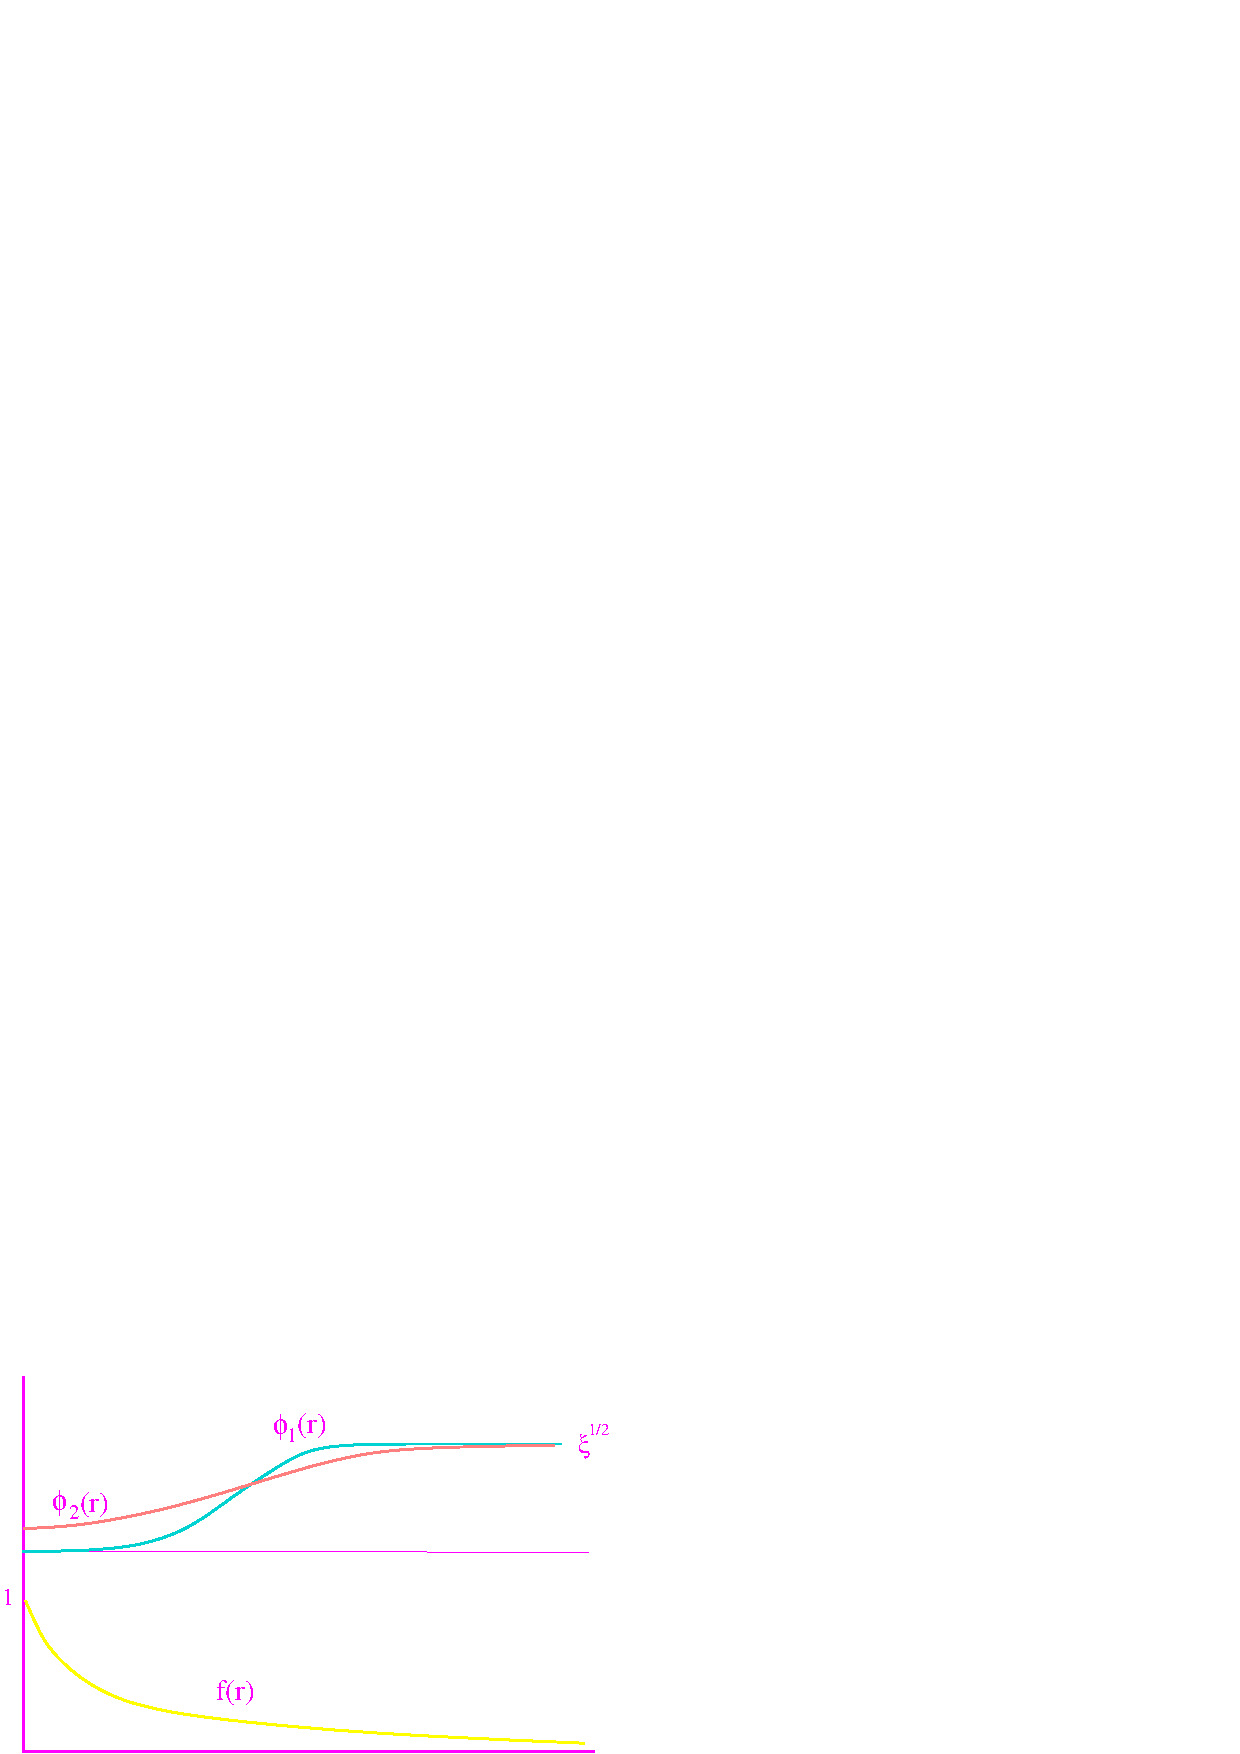
\includegraphics[width=6.0cm]{profiles.pdf}
\end{center}
\begin{align*}
%
	& \phi_1(0) ~~=~~ 0\text, \qquad  \phi_2(0) ~~\neq~~ 0 \\
%
	& f_{NA}(0) ~~=~~ 1\text, \qquad  f(0) ~~=~~ 1\\
%
	\text{and} \\
%
	& \phi_1(\infty) ~~=~~ \sqrt{\xi} \text, \qquad \phi_2(\infty) ~~=~~ \sqrt{\xi} \\
%
	& f_{NA}(\infty) ~~=~~ 0 \text\, \qquad f(\infty) ~~=~~ 0\text.
\end{align*}

\end{slide}

%%%%%%%%%%%%%%%%%%%%%%%%%%%%%%%%%%%%%%%%%%%%%%%%%%%%%%%%%%%%%%%%%%%%%%%%%%%%%%%%%%%%%
%%%%%%%%%%%%%%%%%%%%%%%%%%%%%%%%%%%%%%%%%%%%%%%%%%%%%%%%%%%%%%%%%%%%%%%%%%%%%%%%%%%%%
\begin{slide}
	The profiles satisfy the 1st order BPS equations 
\begin{align*}
%
	\p_r\, \phi_1(r) ~~=~~ & \frac{1}{Nr}\, \lgr f(r) ~+~ (N-1)f_{NA}(r) \rgr \phi_1(r)  \\
%
	\p_r\, \phi_2(r) ~~=~~ & \frac{1}{Nr}\, \lgr f(r) ~-~ f_{NA}(r) \rgr \phi_2(r) \\
%
	\p_r\, f(r)      ~~=~~ & r\, \frac{N g_1^2}{4} \lgr (N-1)\phi_2(r)^2 ~+~ \phi_1(r)^2 ~-~ N\xi \rgr \\
	\p_r\, f_{NA}(r)  ~~=~~ & r\, \frac{g_2^2}{2} \lgr \phi_1(r)^2 ~-~ \phi_2(r)^2 \rgr 
	\text.
\end{align*}

	The tension of the string is 
\[
	T  ~~=~~ 2\pi\, \xi \text.
\]

\end{slide}

%%%%%%%%%%%%%%%%%%%%%%%%%%%%%%%%%%%%%%%%%%%%%%%%%%%%%%%%%%%%%%%%%%%%%%%%%%%%%%%%%%%%%
%%%%%%%%%%%%%%%%%%%%%%%%%%%%%%%%%%%%%%%%%%%%%%%%%%%%%%%%%%%%%%%%%%%%%%%%%%%%%%%%%%%%%
\begin{slide}
	The string orientation $ U $ can be unambigiously parametrized by the modulus $ n^l \in C $:
\[
	\frac{1}{N}\, U \, \lgr \begin{matrix}
				  1  & \ldots & 0 & 0 \\
				  \ldots & \ldots & \ldots & \ldots \\
				  0 & \ldots & 1 & 0  \\
				  0 & 0 & \ldots & -(N-1) 
				\end{matrix} \rgr
			U^{-1}  
	~~=~~
	-\, n^i\,\ov{n}{}_l  ~~+~~ \frac{1}{N}\cdot{\mathlarger{\mathbf{1}}}{}^i_{~l} 
\]
	with a condition
\[
	\ov{n}{}_l \cdot n^l ~~=~~ 1 \text.
\]
	Thus $ n^l $ are \emph{orientational} collective coordinates

	This defines $ 2(N - 1) $ degrees of freedom, since CP(N-1) theory can be obtained from a gauge
	theory, and one phase can be removed

\end{slide}


%%%%%%%%%%%%%%%%%%%%%%%%%%%%%%%%%%%%%%%%%%%%%%%%%%%%%%%%%%%%%%%%%%%%%%%%%%%%%%%%%%%%%
%%%%%%%%%%%%%%%%%%%%%%%%%%%%%%%%%%%%%%%%%%%%%%%%%%%%%%%%%%%%%%%%%%%%%%%%%%%%%%%%%%%%%
\begin{slide}
\vspace*{\fill}
	To find the effective worldsheet model, one needs to substitute the bosonic string solution  $ q^{kA} $,
	$ A_i^{\rm U(1)} $, {\it etc}, 
	depending on the orientational coordinates $ n^l $ into the original action, to calculate
	the so-called \emph{overlap} of the zero-modes

	In a supersymmetric model, one also needs to substitute the fermionic zero-modes which depend
	both on orientational and on fermionic orientational coordinates
\vspace*{\fill}
\end{slide}


%%%%%%%%%%%%%%%%%%%%%%%%%%%%%%%%%%%%%%%%%%%%%%%%%%%%%%%%%%%%%%%%%%%%%%%%%%%%%%%%%%%%%
%%%%%%%%%%%%%%%%%%%%%%%%%%%%%%%%%%%%%%%%%%%%%%%%%%%%%%%%%%%%%%%%%%%%%%%%%%%%%%%%%%%%%
\begin{slide}

	The fermionic zero-modes can be obtained by applying $ \mc{N}=2 $ supersymmetry transformations
	to the bosonic solution $ q^{kA} $.
	For example, the superorientational modes are
\begin{align*}
%
\notag
\overline{\psi}_{\dot{2}Ak} & ~~=~~ \frac{\phi_1^2 ~-~ \phi_2^2}{\phi_2} \cdot n \overline{\xi}_L   \\
%
\notag
\overline{\wt{\psi}}_{\dot{1}}^{kA}  & ~~=~~ - \frac{\phi_1^2 ~-~ \phi_2^2}{\phi_2} \cdot \xi_R \nbar  \\
%
\lambda^{11\ SU(N)} & ~~=~~ i \sqrt{2}\, \frac{ x^1 ~-~ i\, x^2 }{r^2} \frac{\phi_1}{\phi_2} f_N \cdot n \overline{\xi}_L \\
%
\notag
\lambda^{22\ SU(N)} & ~~=~~ - i \sqrt{2}\, \frac{ x^1 ~+~ i\, x^2 }{r^2} \frac{\phi_1}{\phi_2} f_N \cdot \xi_R \nbar 
\end{align*}
	where $ \xir $, $ \xil $ are the \emph{superorientational} collective coordinates
\end{slide}

%%%%%%%%%%%%%%%%%%%%%%%%%%%%%%%%%%%%%%%%%%%%%%%%%%%%%%%%%%%%%%%%%%%%%%%%%%%%%%%%%%%%%
%%%%%%%%%%%%%%%%%%%%%%%%%%%%%%%%%%%%%%%%%%%%%%%%%%%%%%%%%%%%%%%%%%%%%%%%%%%%%%%%%%%%%
\begin{slide}
	In the $\mc{N}=1 $ theory, half of supersymmetry is lost, and with this approach one
	can only recover half of the zero-modes -- the left-handed modes.

	In order to obtain the right-handed modes on has to solve the Dirac equations
\begin{align*}
%
	&
	4\, \frac{i}{g_1^2} \left(\ov{\slashed{\p}} \lambda^{f}_{\rm U(1)} \right)
	+ i\sqrt{2} {\rm Tr} \lgr \ov{\psi} q^f ~+~ \ov{q}{}^f \ov{\wt{\psi}} \rgr 
		- 4 \delta_2^{\ f} \sqrt{\frac{N}{2}}\mu\, \ov{\lambda}{}^{\rm U(1)}_{2} ~=~ 0 
	\\
%
	&
	\frac{i}{g_2^2} \left( \ov{\slashed{\md}}\lambda_{\rm SU(N)}^f \right) 
	~+~ \frac{i}{\sqrt{2}} \lgr \ov{\psi} T^a q^f   ~+~  \ov{q}{}^f T^a \ov{\wt{\psi}} \rgr T^a ~-~ \\
%
	&
	\qquad\qquad\qquad\qquad\qquad\qquad\qquad
		~-~ \delta_2^{\ f}\, \mu\, \ov{\lambda}{}_2^{\rm SU(N)} ~~=~~0
	\\
%
	&  \qquad\qquad\qquad\qquad \ldots
	\\
%
	&  \qquad\qquad\qquad\qquad \ldots
\end{align*}
\end{slide}

%%%%%%%%%%%%%%%%%%%%%%%%%%%%%%%%%%%%%%%%%%%%%%%%%%%%%%%%%%%%%%%%%%%%%%%%%%%%%%%%%%%%%
%%%%%%%%%%%%%%%%%%%%%%%%%%%%%%%%%%%%%%%%%%%%%%%%%%%%%%%%%%%%%%%%%%%%%%%%%%%%%%%%%%%%%
\begin{slide}
	The equations are not solveable exactly, and one can resolve them in 
	a limit of small or large $ \mu $. 

	It turns out that the right-handed zero-modes have $ 1/r $-tails
\[
	\ov{\wt{\psi}}{}_{\dot{1}}  ~~\simeq~~  \frac{\phi_2}{r}\, n\nbar\, \zr  ~~\sim~~ \frac{\sqrt{\xi}}{r}\, n\nbar\, \zr
\]

	These long-range tails reflect the presence of the Higgs branch.

	One expects to be able to substitute these zero-modes into the microscopic action in order to 
	obtain the effective sigma model
\end{slide}

%%%%%%%%%%%%%%%%%%%%%%%%%%%%%%%%%%%%%%%%%%%%%%%%%%%%%%%%%%%%%%%%%%%%%%%%%%%%%%%%%%%%%
%%%%%%%%%%%%%%%%%%%%%%%%%%%%%%%%%%%%%%%%%%%%%%%%%%%%%%%%%%%%%%%%%%%%%%%%%%%%%%%%%%%%%
\begin{slide}
	It turns out that CP(N-1) does not admit $\mc{N}=(0,2)$ generalization.

	However, the model we are deriving is not exactly CP(N-1)
\begin{align*}
	\mc{L}_{CP(N-1)} & ~~=~~ 
		\left|\p_k n \right|^2  ~+~ \left(\ov{n}\p_k n\right)^2  
		~+~ \ov{\xi}{}_L\, i\p_R\, \xi_L  ~+~ \ov{\xi}{}_R\, i\p_L\,  \xi_R 
	\\
%
	&
	~~~-~
	i \left(\nbar\p_R n\right)\, \bxil\xil ~-~ i \left(\nbar\p_Ln\right) \, \bxir\xir 
	\\
%
	&
	~~~+~
		\bxil \xir \bxir \xil ~-~ \bxir \xir \bxil \xil
\end{align*}
\[
	\nbar{}_l n^l ~~=~~ 1\text, \qquad \nbar_l \xi^l ~~=~~ \ov{\xi}{}_l n^l ~~=~~ 0\text,
\]
\[
	\p_R ~~=~~ \p_0 ~+~ i\p_1 \text, \qquad\qquad \p_L ~~=~~ \p_0 ~-~ i\p_1
\]

	Our theory possesses supertranslational modes $ \zr $ which mix with the orientational
	modes
\end{slide}

%%%%%%%%%%%%%%%%%%%%%%%%%%%%%%%%%%%%%%%%%%%%%%%%%%%%%%%%%%%%%%%%%%%%%%%%%%%%%%%%%%%%%
%%%%%%%%%%%%%%%%%%%%%%%%%%%%%%%%%%%%%%%%%%%%%%%%%%%%%%%%%%%%%%%%%%%%%%%%%%%%%%%%%%%%%
\begin{slide}
	Therefore, our model is extended with $ \zr $, and it was argued by Edalati and Tong that
	it has to be $ CP(N-1) \times C $ sigma model

	Based on $\mc{N}=(0,2)$ superfield formalism, they were able to build the $\mc{N}=(0,2) $
	$ CP(N-1) \times C $ sigma model

	The major ingredient in the (modification of the) CP(N-1) model is the quadratic superpotential
\[
	\hat{\mc{W}}{}_{1+1}  ~~=~~ \frac{1}{2} \, \delta \, \Sigma^2
\]
	which reflects the presence of $ \mu\mc{A}^2 $ in the microscopic theory.
	Also the right-handed constraints are now modified
\[
	\bxir \cdot n   ~~\neq~~ 0 \text, \qquad\qquad  \nbar \cdot \xir ~~\neq~~0
\]
\end{slide}


%%%%%%%%%%%%%%%%%%%%%%%%%%%%%%%%%%%%%%%%%%%%%%%%%%%%%%%%%%%%%%%%%%%%%%%%%%%%%%%%%%%%%
%%%%%%%%%%%%%%%%%%%%%%%%%%%%%%%%%%%%%%%%%%%%%%%%%%%%%%%%%%%%%%%%%%%%%%%%%%%%%%%%%%%%%
\begin{slide}
	
	The latter constraints can be restored via a shift
\begin{align*}
%
	\bxir ~~\to~~ \bxir ~-~ \frac{m_W}{\sqrt{2}}\, \delta\,\zeta_R\ov{n} \\
%
	\xi_R ~~\to~~ \xi_R ~-~ \frac{m_W}{\sqrt{2}}\, \ov{\delta}\, \bzr n~
\end{align*}

	This, together with the quadratic superpotential 
\[
	\hat{\mc{W}}{}_{1+1}  ~~=~~ \frac{1}{2} \, \delta \, \Sigma^2
\]
	leads to mixing of supertranslational and superorientational modes $ \zr $ and $ \xir $.

\end{slide}


%%%%%%%%%%%%%%%%%%%%%%%%%%%%%%%%%%%%%%%%%%%%%%%%%%%%%%%%%%%%%%%%%%%%%%%%%%%%%%%%%%%%%
%%%%%%%%%%%%%%%%%%%%%%%%%%%%%%%%%%%%%%%%%%%%%%%%%%%%%%%%%%%%%%%%%%%%%%%%%%%%%%%%%%%%%
\begin{slide}
	In terms of components, upon the elimination 
	of all the auxiliary fields the $\mc{N}=(0,2)$ takes the form
\begin{align*}
%
\notag
\mc{L}_{1+1}^{(0,2)} &~=~ 
	\bzr\, i\p_L\, \zr ~~+~~ \dots ~~+~~
	\\
%
\notag
	&
	+~~
	\left|\p n\right|^2 ~~+~~ \left(\ov{n}\p_k n\right)^2 ~~+~~
	\bxir \, i\p_L \, \xir  ~~+~~ \bxil \, i\p_R \, \xil 
	\\
%
\notag
	&
	-~~
	i \left(\ov{n}\p_L n\right)\, \bxir \xir ~~-~~ 
	i \left(\ov{n}\p_R n\right)\, \bxil \xil 
	\\
%
\notag
	&
	-~~
	\gamma\, (i\p_L\nbar) \xir\zr ~~-~~ \ov{\gamma}\, \bxir (i\p_L n) \bzr ~~+~~
	|\gamma|^2\, \bxil\xil \bzr\zr 
	\\
%
\notag
	&
	+~~ 
	\left( 1 \;-\; |\gamma|^2 \right)\, \bxil\xir \bxir\xil  
	~~-~~ \bxil\xil \bxir\xir
\end{align*}
	where
\[
	\gamma ~~=~~ \frac { \sqrt{2}\,\delta } { \sqrt{ 1 +  2 |\delta|^2 } }~.
\]

	Our goal is to find $ \gamma $ (or $ \delta $) in terms of the microscopic parameter $ \mu $
\end{slide}

%%%%%%%%%%%%%%%%%%%%%%%%%%%%%%%%%%%%%%%%%%%%%%%%%%%%%%%%%%%%%%%%%%%%%%%%%%%%%%%%%%%%%
%%%%%%%%%%%%%%%%%%%%%%%%%%%%%%%%%%%%%%%%%%%%%%%%%%%%%%%%%%%%%%%%%%%%%%%%%%%%%%%%%%%%%
\begin{slide}

	We calculate the \emph{bifermionic mixing} term 
\[
	-~\gamma\, (i\p_L\nbar) \xir\zr
\]
	from the microscopic theory

	The result is
\[
	\delta~~=~~ {\rm const} \cdot \sqrt{\ln\, \frac{g_2^2\mu}{m_W}}~,
	\qquad\qquad \text{as $\mu ~\to~ \infty$}~.
\]
	and
\[
	\delta~~=~~ {\rm const} \cdot \frac{g^2\mu}{m_W} \qquad\qquad \text{small $\mu$.}
\]
\end{slide}

%%%%%%%%%%%%%%%%%%%%%%%%%%%%%%%%%%%%%%%%%%%%%%%%%%%%%%%%%%%%%%%%%%%%%%%%%%%%%%%%%%%%%
%%%%%%%%%%%%%%%%%%%%%%%%%%%%%%%%%%%%%%%%%%%%%%%%%%%%%%%%%%%%%%%%%%%%%%%%%%%%%%%%%%%%%
\begin{slide}

	We do a similar calculation in the $M$-model
\[
	\mc{L}_{\rm quark} ~~=~~ \int d^2\theta\, d^2\ov{\theta}~  \frac{2}{h}\, {\rm Tr}\, \ov{M}M  ~~+~~
			\int d^2\theta~ Q M\wt{Q}
\]

	Once there is finite $h$, the Higgs branch is lifted and $\mu$ can
	be taken to infinity

	In this case one needs the zero-modes of the fermionic $M$ and quark fields

	By solving Dirac equations (in the small $ h $ limit), and calculating the overlap
\[
	\delta ~~=~~ \text{const} \cdot \sqrt{\ln\, g_2^2 / h}
\]

	Here $ h $ needs to be small, but finite, no need to take it to zero

\end{slide}

%%%%%%%%%%%%%%%%%%%%%%%%%%%%%%%%%%%%%%%%%%%%%%%%%%%%%%%%%%%%%%%%%%%%%%%%%%%%%%%%%%%%%
%%%%%%%%%%%%%%%%%%%%%%%%%%%%%%%%%%%%%%%%%%%%%%%%%%%%%%%%%%%%%%%%%%%%%%%%%%%%%%%%%%%%%
\begin{slide}
{
\usefont{T1}{ptm}{m}{n}\fontsize{20pt}{20pt}\selectfont
\begin{center} 
	Conclusion
\end{center}
}
\vspace*{\fill}
\begin{itemize}
\item
	Supersymmetric QCD theories with $ \mc{N}>1 $ can be brought into the confinement
	regime for the monopoles

\item
	$ \sunu $ with $ N $ flavours

\item
	Confinement is essentially \emph{non-abelian} (non-abelian strings)

\item
	Monopoles can be studied as kinks of the 2-dimensional worldsheet model: in particular
	the masses match

\end{itemize}
\vspace*{\fill}
\end{slide}

%%%%%%%%%%%%%%%%%%%%%%%%%%%%%%%%%%%%%%%%%%%%%%%%%%%%%%%%%%%%%%%%%%%%%%%%%%%%%%%%%%%%%
%%%%%%%%%%%%%%%%%%%%%%%%%%%%%%%%%%%%%%%%%%%%%%%%%%%%%%%%%%%%%%%%%%%%%%%%%%%%%%%%%%%%%
\begin{slide}
\vspace*{\fill}
\begin{itemize}
\item	
	Attempts to break supersymmetry to $ \mc{N}=1 $ lead to massless modes on the Higgs branch

\item
	One can introduce a meson field which gives quark a dynamical mass and lift the Higgs branch

\item
	The worldsheet dynamics of the non-abelian strings is described by $ C\times CP(N-1) $
\end{itemize}
\vspace*{\fill}
\end{slide}


%%%%%%%%%%%%%%%%%%%%%%%%%%%%%%%%%%%%%%%%%%%%%%%%%%%%%%%%%%%%%%%%%%%%%%%%%%%%%%%%%%%%%
%%%%%%%%%%%%%%%%%%%%%%%%%%%%%%%%%%%%%%%%%%%%%%%%%%%%%%%%%%%%%%%%%%%%%%%%%%%%%%%%%%%%%
\begin{slide}
%\vspace*{\fill}
\begin{itemize}
\item
	Considering it as a modification of the $ CP(N-1) $ model, the modification parameter
	of the 2-d superpotential is given as 
\[
	\delta~~=~~ {\rm const} \cdot \sqrt{\ln\, \frac{g_2^2\mu}{m_W}}~,
	\qquad\qquad \text{as $\mu ~\to~ \infty$}
\]
	in softly broken $\mc{N}=2 ~\to~ \mc{N}=1 $ SQCD, and
\[
	\delta ~~=~~ \text{const} \cdot \sqrt{\ln\, g_2^2 / h}~,
	\qquad\qquad \text{as $h ~\to~ 0$}
\]
	in the $M$-model
%\[
%	\delta~~=~~ {\rm const} \cdot \frac{g^2\mu}{m_W} \qquad\qquad \text{small $\mu$.}
%\]
\end{itemize}
\end{slide}


%%%%%%%%%%%%%%%%%%%%%%%%%%%%%%%%%%%%%%%%%%%%%%%%%%%%%%%%%%%%%%%%%%%%%%%%%%%%%%%%%%%%%
%%%%%%%%%%%%%%%%%%%%%%%%%%%%%%%%%%%%%%%%%%%%%%%%%%%%%%%%%%%%%%%%%%%%%%%%%%%%%%%%%%%%%
\begin{slide}
\vspace*{\fill}
\begin{itemize}
\item
	The next step is to introduce masses to the quark fields ($\Delta m_{AB}$)

\item 
	The massive heterotic worldsheet model is already being considered

\item 
	Another direction of extension is to consider $ N_F > N_c $, where the
	strings become semi-local, and size moduli appear on the string worldsheet
	(simultaneously an extension of the Non-Abelan duality to the $\mc{N}=1$
	case)
\end{itemize}	

\begin{center}
\usefont{T1}{ptm}{m}{n}\fontsize{10pt}{10pt}\selectfont
	Work done in collaboration with Alexei Yung and Mikhail Shifman, FTPI, Minnesota
\end{center}
\vspace*{\fill}
\end{slide}


\end{document}
\endinput

%%
%% End of file `talk.tex'.
